\documentclass[tikz,border=15pt]{standalone}
\usepackage[T1]{fontenc}
\usepackage{lmodern}
\usetikzlibrary{arrows.meta,positioning,fit,backgrounds,calc,
    decorations.pathreplacing}

\definecolor{llmblue}{HTML}{1565C0}
\definecolor{replorange}{HTML}{E65100}
\definecolor{finalgreen}{HTML}{2E7D32}
\definecolor{printpurple}{HTML}{7B1FA2}
\definecolor{subllmteal}{HTML}{00838F}
\definecolor{loopgray}{HTML}{455A64}
\definecolor{togethergray}{HTML}{37474F}
\definecolor{nsbg}{HTML}{FFF3E0}
\definecolor{llmbg}{HTML}{E8F0FE}
\definecolor{loopbg}{HTML}{ECEFF1}

\begin{document}
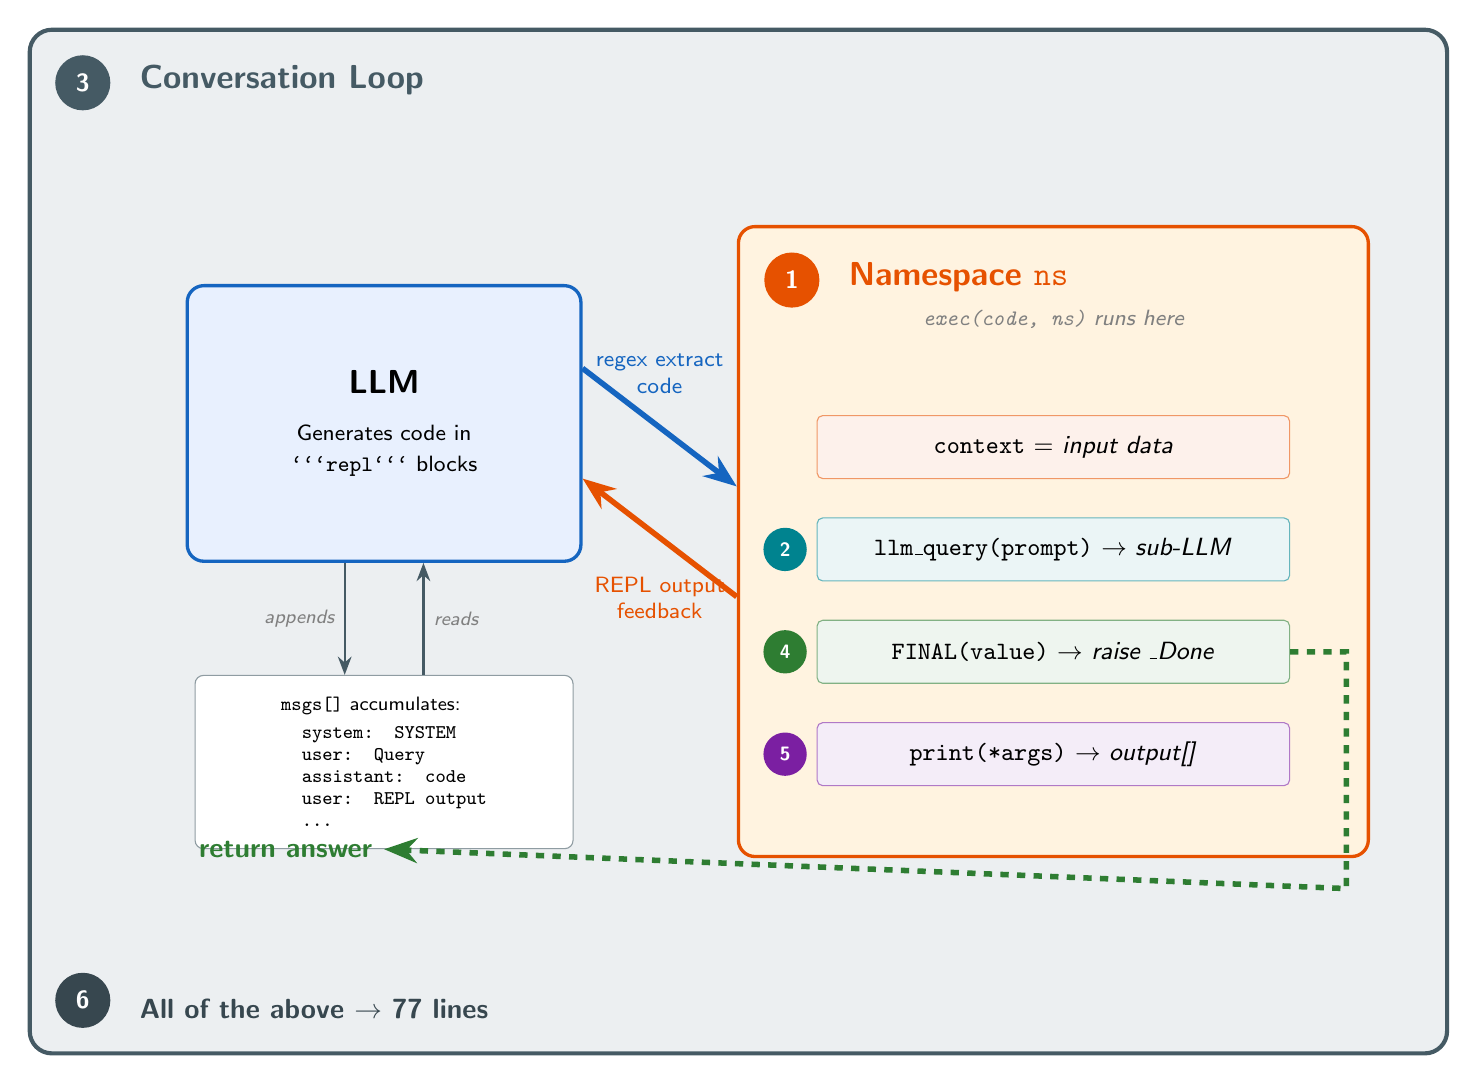
\begin{tikzpicture}[
    >=Stealth,
    font=\sffamily\small,
    stepbadge/.style={circle, minimum size=0.7cm, font=\sffamily\bfseries\small,
        text=white, inner sep=0pt},
    smallbadge/.style={circle, minimum size=0.55cm, font=\sffamily\bfseries\scriptsize,
        text=white, inner sep=0pt},
    nsentry/.style={draw=#1!60, fill=#1!8, rounded corners=2pt,
        minimum width=6cm, minimum height=0.8cm, align=center,
        font=\sffamily\small},
    ann/.style={font=\sffamily\scriptsize\itshape, text=black!50},
]

% =====================================================
% Step 3: Conversation loop — outer frame
% =====================================================
\node[draw=loopgray, line width=1.5pt, rounded corners=8pt,
    fill=loopbg, minimum width=18cm, minimum height=13cm]
    (loopframe) at (0, 0) {};

\node[stepbadge, fill=loopgray]
    at ([xshift=0.7cm, yshift=-0.7cm]loopframe.north west) {3};
\node[anchor=north west, font=\sffamily\bfseries\large,
    text=loopgray] at ([xshift=1.3cm, yshift=-0.35cm]loopframe.north west)
    {Conversation Loop};

% =====================================================
% LLM box (left side)
% =====================================================
\node[draw=llmblue, line width=1.2pt, rounded corners=6pt,
    fill=llmbg, minimum width=5cm, minimum height=3.5cm,
    align=center] (llm) at (-4.5, 1.5)
    {\textbf{\large LLM}\\[6pt]
     {\footnotesize Generates code in}\\
     {\footnotesize\texttt{```repl```} blocks}};

% =====================================================
% Namespace box — Step 1 (right side)
% =====================================================
\node[draw=replorange, line width=1.2pt, rounded corners=6pt,
    fill=nsbg, minimum width=8cm, minimum height=8cm]
    (nsframe) at (4, 0) {};

\node[stepbadge, fill=replorange]
    at ([xshift=0.7cm, yshift=-0.7cm]nsframe.north west) {1};
\node[anchor=north west, font=\sffamily\bfseries\large,
    text=replorange] at ([xshift=1.3cm, yshift=-0.35cm]nsframe.north west)
    {Namespace \texttt{ns}};

\node[font=\sffamily\footnotesize\itshape, text=black!50]
    at ([yshift=-1.2cm]nsframe.north) {\texttt{exec(code, ns)} runs here};

% --- Namespace entries ---

\node[nsentry=replorange] (ctx) at (4, 1.2)
    {\texttt{context} = \textit{input data}};

\node[nsentry=subllmteal] (llmq) at (4, -0.1)
    {\texttt{llm\_query(prompt)} $\rightarrow$ \textit{sub-LLM}};
\node[smallbadge, fill=subllmteal]
    at ([xshift=-0.4cm]llmq.west) {2};

\node[nsentry=finalgreen] (fin) at (4, -1.4)
    {\texttt{FINAL(value)} $\rightarrow$ \textit{raise \_Done}};
\node[smallbadge, fill=finalgreen]
    at ([xshift=-0.4cm]fin.west) {4};

\node[nsentry=printpurple] (prn) at (4, -2.7)
    {\texttt{print(*args)} $\rightarrow$ \textit{output[]}};
\node[smallbadge, fill=printpurple]
    at ([xshift=-0.4cm]prn.west) {5};

% =====================================================
% Arrows: LLM ↔ Namespace (parallel, well-spaced)
% =====================================================

\draw[->, llmblue, line width=2pt]
    ([yshift=0.7cm]llm.east) -- ([yshift=0.7cm]nsframe.west)
    node[midway, above=8pt, font=\sffamily\footnotesize, align=center]
    {regex extract\\code};

\draw[->, replorange, line width=2pt]
    ([yshift=-0.7cm]nsframe.west) -- ([yshift=-0.7cm]llm.east)
    node[midway, below=10pt, font=\sffamily\footnotesize, align=center]
    {REPL output\\feedback};

% =====================================================
% msgs[] box (below LLM)
% =====================================================
\node[draw=loopgray!60, fill=white, rounded corners=3pt,
    minimum width=4.8cm, minimum height=2.2cm, align=left,
    font=\sffamily\scriptsize] (msgs) at (-4.5, -2.8)
    {\texttt{msgs[]} accumulates:\\[2pt]
    \texttt{\ \ system: SYSTEM}\\
    \texttt{\ \ user: Query}\\
    \texttt{\ \ assistant: code}\\
    \texttt{\ \ user: REPL output}\\
    \texttt{\ \ ...}};

\draw[->, loopgray, thick]
    ([xshift=-0.5cm]llm.south) -- ([xshift=-0.5cm]msgs.north)
    node[midway, left, ann] {appends};
\draw[->, loopgray, thick]
    ([xshift=0.5cm]msgs.north) -- ([xshift=0.5cm]llm.south)
    node[midway, right, ann] {reads};

% =====================================================
% FINAL exit arrow — exits right, curves down and along bottom
% =====================================================
\draw[->, finalgreen, line width=2pt, dashed]
    (fin.east) -- ([xshift=-0.3cm]nsframe.east |- fin)
    -- ([xshift=-0.3cm, yshift=-0.5cm]nsframe.east |- msgs.south)
    -- (-4.5, -4.7 |- msgs.south)
    node[at end, left, font=\sffamily\bfseries,
        text=finalgreen] {return answer};

% =====================================================
% Step 6 label
% =====================================================
\node[stepbadge, fill=togethergray]
    at ([xshift=0.7cm, yshift=0.7cm]loopframe.south west) {6};
\node[anchor=south west, font=\sffamily\bfseries,
    text=togethergray]
    at ([xshift=1.3cm, yshift=0.35cm]loopframe.south west)
    {All of the above $\rightarrow$ 77 lines};

\end{tikzpicture}
\end{document}
